\chapter{Use Case: \acs{PaTAS} Applied to 5G Network Energy Management}
\label{chap:usecase}
\todo{rework c4, improve it}
\todo{split figure}
\todo{ackn that this is not the best model given the temporal nature of the problem an LSTM might be better}
\noindent
The previous chapters introduced the theoretical foundations and system architecture required to perform trust assessment in \ac{NN} systems. In particular, \cref{chap:ovl,chap:dataset-trust,chap:patas} introduced the \ac{PaTAS} architecture for parallel trust assessment through the whole \ac{NN} system pipeline. This chapter demonstrates how these contributions apply in practice through a concrete use case in 5G network energy management. The objective is not to introduce new theoretical contributions, but rather to illustrate how the proposed methodology can be applied to assess trustworthiness within a realistic \ac{ML} scenario. By instantiating the full trust assessment pipeline, from trust proposition definition to evidence collection, opinion quantification, and reasoning, we show how the framework can support practical decision-making regarding the trustworthiness of \ac{ML} systems.


\section{Introduction and Motivation}
\label{sec:intro}
5G network energy management is a trust-critical domain: decisions are automated, data arrives from heterogeneous hardware, and errors propagate directly into resource allocation. In this work, we evaluate \ac{PaTAS} using a real-world dataset from 5G network energy consumption monitoring\cite{netop_5g_energy_2026}. This scenario is particularly suited for evaluating \ac{PaTAS} because:
\begin{itemize}
    \item Data comes from heterogeneous infrastructure spanning more than 1,000 base stations with 12 different hardware types, creating natural variation in measurement reliability.
    \item Labels are derived via automated quantile binning, introducing systematic artifacts independent of measurement noise.
    \item Both features and labels carry inherent noise and uncertainty that must be explicitly modeled for trustworthy predictions.
    \item The task has direct practical significance: accurate energy modeling is essential for optimizing resource allocation in next-generation wireless networks.
\end{itemize}

Through this use case, we answer four questions:
\begin{enumerate}
    \item How should trust opinions be assigned to real-world data?
    \item How do trust opinions propagate through the network during training?
    \item Does the trust signal produced by \ac{PaTAS} reliably indicate prediction correctness under noise?
    \item How does \ac{PaTAS}-based per-prediction trust relate to a global calibration-trust assessment of the same model?
\end{enumerate}

The remainder of this chapter is organized as follows. \Cref{sec:dataset} describes the 5G energy dataset and experimental setup. \Cref{sec:trust_quantification} presents the trust quantification methodology for features and labels. \Cref{sec:trust_propagation} describes how trust opinions propagate through the network during training. \Cref{sec:noise_robustness} evaluates PaTAS as a confidence signal under noise. \Cref{sec:calibration_quantification} compares per-prediction trust with global calibration trust. \Cref{sec:discussion} discusses implications and limitations, and \Cref{sec:conclusion} concludes.


\section{Dataset and Experimental Setup}
\label{sec:dataset}
\subsection{The 5G Energy Dataset}
\label{sec:5g_dataset}

The 5G energy consumption dataset consists of operational measurements collected from a large-scale production network deployment over an 8-day period. It comprises measurements from more than 1,000 \acp{RRU} and \acp{AAU} spanning 12 distinct hardware product types, collected at hourly granularity. The dataset contains close to 100,000 base-station-level samples, providing substantial statistical power for evaluating trust quantification and propagation.


\subsubsection{Data Structure and Collection}
\label{sec:data_structure}

The dataset is organized into three coordinated CSV files that capture complementary aspects of network operation. \Cref{tab:data_files} summarizes these files.

\begin{table}[h]
\centering
\caption{5G Energy Dataset Files and Fields}
\label{tab:data_files}
\begin{tabular}{|l|p{3cm}|p{5cm}|}
\hline
\textbf{File} & \textbf{Content} & \textbf{Key Fields} \\
\hline
BSinfo.csv & Static base station and cell configuration & BS, CellName, RUType, Bandwidth, Frequency, Antennas, TXpower \\
\hline
CLstat.csv & Hourly cell-level operational status & Time, BS, CellName, Load, EnergySavingMode (1 to 6) \\
\hline
ECstat.csv & Hourly energy consumption per base station & Time, BS, Energy \\
\hline
\end{tabular}
\end{table}


\subsubsection{Feature Engineering and Label Definition}
\label{sec:features_labels}

Features are constructed through a multi-stage preprocessing pipeline. First, the three CSV files are joined on $(Time, BS, CellName)$. Cell-level measurements are aggregated to base station level by computing the mean of numerical features and the mode of categorical features. The resulting feature vector has 26 dimensions:

\begin{itemize}
    \item Load: 1 feature (cell utilization factor)
    \item Energy-saving mode: 6 features (ESMode1 to ESMode6, binary/ordinal indicators)
    \item Hardware characteristics: 5 features (Bandwidth, Frequency, Antennas, TXpower, NumCells)
    \item Equipment type: 14 features (one-hot encoding of 12 RUType variants plus 2 Modes)
\end{itemize}

All numerical features are standardized (mean approximately 0, standard deviation approximately 1) before use.

The target label is energy consumption discretized into three classes via quantile binning. Bin boundaries are computed independently for each base station and time window to reflect domain expectations about load-dependent energy usage. The three classes are Low (at or below the 33rd percentile), Medium (between 33rd and 66th percentile), and High (above the 66th percentile). Labels are created via automated quantile binning, which is computationally efficient but introduces natural label noise: measurement errors and temporal shifts cause static quantile boundaries to misalign with true energy classes. 
The impact of this natural noise is compounded by the controlled noise we 
introduce experimentally, as described in \Cref{sec:noise_injection}.

\subsection{Model Configuration}
\label{sec:model_config}

We train a 2-layer \ac{MLP} with architecture $26 \to 32 \to 3$ to learn the energy classification task. We deliberately choose a simple architecture for three reasons: (1) it balances model capacity with interpretability, allowing clear observation of trust phenomena without the confounding of deep feature hierarchies; (2) it aligns with prior work on \ac{PaTAS} \cite{patas_chapter}, which has focused on shallow networks to enable controlled analysis of trust propagation; and (3) simple models provide a conservative baseline for evaluating whether trust reasoning adds value even in the simplest case, with the expectation that deeper networks may show larger benefits.

All neurons use ReLU hidden activations and softmax output activation. Training uses stochastic gradient descent with a fixed learning rate of $0.05$ and batch size of 64 for 10 epochs. Batch normalization and dropout are not used, in order to maintain transparency in trust propagation and avoid confounding factors in our analysis.

Parameter trust opinions are initialized to the vacuous state $(b=0, d=0, u=1)$ in both layers, representing complete ignorance before training. The \ac{PaTAS} and \ac{NN} run as separate processes communicating over a local \acs{TCP} socket, enabling modular integration of trust reasoning without modifying the underlying \ac{NN}'s forward or backward pass.


\subsection{Noise Injection Strategy}
\label{sec:noise_injection}

To evaluate \ac{PaTAS} under realistic data quality variation, we inject controlled noise into both features and labels. Feature noise is injected per-sample: each training sample $i$ independently draws its own noise level $\sigma_i$ from a uniform distribution:

\[
\sigma_i \sim \text{Uniform}(0, \sigma_{\max}), \quad i = 1, 2, \ldots, n
\]

Feature noise for sample $i$ is then additive Gaussian:

\[
\tilde{X}_i = X_i + \epsilon_i, \quad \epsilon_i \sim \mathcal{N}(0, \sigma_i \cdot \text{std}(X))
\]

To simulate label noise at controlled levels, we corrupt a fraction $p$ of all training labels by randomly reassigning them to an incorrect class, chosen uniformly from the remaining two classes. This controlled corruption mimics realistic label noise sources such as automated binning failures or inconsistent annotations, while keeping $p$ known by construction so that it can be used directly to compute the label trust opinion We conduct each experiment $N_{\text{RUNS}} = 5$ times with independent random number generator seeds. Results are averaged to obtain stable mean and standard deviation estimates.

\subsection{Experimental Configurations and Baselines}
\label{sec:configs}

We compare two configurations, summarized in \Cref{tab:configs}.

\begin{table}[h]
\centering
\caption{Experimental configurations. Both configurations use the same underlying neural network and dataset; they differ only in whether trust opinions are computed and propagated in parallel.}
\label{tab:configs}
\begin{tabular}{|l|p{3.5cm}|p{3.5cm}|c|}
\hline
\textbf{Config} & \textbf{Feature trust at training} & \textbf{Label trust at training} & \textbf{Runs} \\
\hline
nn & None (baseline NN) & None & 5 \\
\hline
ptas-percal & Per-sample $\sigma_i$ calibration & flip probability $p$ & 5 \\
\hline
\end{tabular}
\end{table}

The \textbf{nn} baseline is a standard neural network without any trust reasoning. It establishes the underlying classification performance and serves as the reference for evaluating \ac{PaTAS}, which does not modify the \ac{NN}'s predictions but provides a complementary trust signal.

The \textbf{ptas-percal} configuration runs \ac{PaTAS} alongside the same \ac{NN} with per-sample heterogeneous trust. Each training sample $i$ has its trust opinion computed as $\text{feature\_noise\_to\_trust}(\sigma_i)$, with $\sigma_i$ drawn as described above. The \ac{PaTAS} looks up $\sigma_i$ by batch index on-the-fly, constructing heterogeneous trust matrices where each row carries distinct belief, disbelief, and uncertainty values. Label trust is computed from the flip probability $p$ via $\text{label\_noise\_to\_trust}(p)$.

\paragraph{Training versus evaluation trust opinions.}
During training, feature trust is heterogeneous (per-sample $\sigma_i$) to reflect the realistic situation where different samples have different reliability. During evaluation, we report \ac{PaTAS} as a function of a single $\sigma_{\text{rel}}$ value, computed by evaluating $\text{feature\_noise\_to\_trust}(\sigma_{\text{rel}})$ uniformly across test samples. This allows controlled comparison of PaTAS behavior under specific noise levels without confounding from per-sample variation. The training-time heterogeneity ensures the network has been exposed to a realistic mix of sample qualities; the evaluation-time uniformity isolates the effect of a given noise condition.


\subsection{Experiments, Training and Evaluation Protocol}
\label{sec:exp_axes}

We evaluate the system along two primary axes:

\begin{enumerate}
    \item \textbf{Feature noise:} $\sigma_{\text{rel}} \in \{0.0, 0.1, 0.3, 0.5\}$ with label flip probability $p = 0$.
    \item \textbf{Combined noise:} Selected pairs $(\sigma_{\text{rel}}, p) \in \{(0.1, 0.05), (0.3, 0.15), (0.5, 0.30)\}$.
\end{enumerate}

For each condition, both \textbf{nn} and \textbf{ptas-percal} are run five times. Reported results are means with standard deviations across runs. 

The pairing of feature and label noise levels is chosen to reflect realistic scenarios where data quality degrades on multiple dimensions simultaneously. At higher feature noise levels $\sigma_{rel}$, we pair correspondingly higher label flip rates $p$ to simulate the expectation that measurement degradation and labeling errors co-occur in production systems.

\paragraph{Training loop.} 
At each training step, the \ac{NN} sends batches of size 64 to the \ac{PaTAS} along with batch indices. The \ac{PaTAS}  retrieves the per-sample trust opinions for that batch and propagates them through the \acf{TNN} in parallel with the standard \ac{NN}'s forward and backward pass. After training, test-time \ac{PaTAS} opinions are computed on the held-out test set under each evaluation condition. We report:
\begin{itemize}
    \item Final test accuracy of the baseline \ac{NN}.
    \item Learning curves showing epoch-wise progression.
    \item \ac{PaTAS} opinion masses $(b, d, u)$ on the \ac{NN}'s predicted class, separated by whether the prediction is correct.
    \item Selective-prediction coverage and accuracy under \ac{PaTAS}-based and softmax-based filters.
\end{itemize}


\section{Trust Assessment: Assigning Opinions to Data}
\label{sec:trust_quantification}

We quantify trust opinions by mapping noise characteristics directly to binomial opinion components $(b, d, u)$ using two domain-specific functions: one for feature noise, one for label noise. This approach embeds the semantic distinction between random measurement variability and systematic labeling errors into the opinion structure itself.


\subsection{Feature Trust Quantification}
\label{sec:feature_trust_quantification}

We define the mapping from noise level to uncertainty as the noise-to-information ratio. Intuitively, a noisy measurement carries less information relative to the signal it is meant to convey. We formalize this by treating $\sigma_{\text{rel}}^2$ as the noise power and 1 as the unit signal power. Since $\sigma_{\text{rel}} < 1$ by construction (noise is always smaller than the signal after z-standardization), the raw ratio $\sigma_{\text{rel}}^2 / (1 + \sigma_{\text{rel}}^2)$ only reaches 0.5 at its maximum ($\sigma_{\text{rel}} = 1$), leaving the upper half of the uncertainty range $[0, 1]$ unreachable. We therefore apply a factor of 2 to rescale the mapping to the full $[0, 1]$ interval:

\begin{equation}
u = \frac{2\sigma_{\text{rel}}^2}{1 + \sigma_{\text{rel}}^2}
\label{eq:feature_u}
\end{equation}

This is consistent with our z-standardization of features in 
\Cref{sec:features_labels}: after standardization, the signal variance is 1 
by construction, making $\sigma_{\text{rel}}^2 / (1 + \sigma_{\text{rel}}^2)$ directly interpretable as the noise-to-signal ratio. 

The remaining mass $1 - u$ is distributed between belief and disbelief (Constant-Uncertainty Quantification in \cref{chap:Trust_method}). Positive and negative evidence are taken as:
\begin{equation}
r = 1 - \sigma_{\text{rel}}, \quad s = \sigma_{\text{rel}}
\end{equation}

and normalized by $\gamma = (1 - u) / (r + s) = 1 - u$, giving:

\begin{equation}
b = (1 - \sigma_{\text{rel}}) (1 - u), \quad d = \sigma_{\text{rel}} (1 - u).
\label{eq:feature_bd}
\end{equation}

The rescaled mapping satisfies three desirable properties:
\begin{itemize}
    \item \textbf{Boundary correctness}: at $\sigma_{\text{rel}} = 0$ (no noise), 
    $u = 0$, yielding the fully-trusted opinion $(1, 0, 0)$; at 
    $\sigma_{\text{rel}} = 1$ (noise power equals signal power), $u = 1$, 
    yielding the vacuous opinion $(0, 0, 1)$.
    \item \textbf{Monotonicity}: $u$ increases strictly with $\sigma_{\text{rel}}$, 
    ensuring that higher noise always produces more uncertainty.
    \item \textbf{Boundedness}: $u \in [0, 1]$ for all $\sigma_{\text{rel}} \in [0, 1]$, 
    guaranteeing a valid opinion at every noise level within the operating range.
\end{itemize}

Moreover, as measurement noise increases, uncertainty grows as the dominant component, while both belief and disbelief shift: belief decreases from 1 toward 0, and disbelief increases from 0 toward a maximum at $\sigma_{\text{rel}} = 0.5$ before both collapse as $u \to 1$. The net effect is uncertainty-dominant: for $\sigma_{\text{rel}} \leq 1$, uncertainty is always the largest single component, reflecting that noisy measurements reduce confidence without implying systematic deception.




\subsection{Label Trust Quantification}
\label{sec:label_trust_quantification}

Label noise from automated binning represents class-flipping errors, where a fraction $p$ of labels are systematically reassigned to the wrong class. Unlike random measurement noise, label flipping is a failure mode of the labeling process itself, producing a disbelief-dominant opinion.

We quantify label trust through a direct linear mapping of flip rate to disbelief:

\begin{equation}
b = 1 - p, \quad d = p, \quad u = 0.
\label{eq:label_bdu}
\end{equation}

At $p = 0$ (clean labels), the opinion is $(1, 0, 0)$ (fully trusted). As the flip rate increases, belief decreases linearly while disbelief rises symmetrically. At $p = 1.0$, the opinion becomes $(0, 1, 0)$, indicating that the labels are reliably wrong. 

The absence of uncertainty ($u = 0$) reflects a deliberate modeling choice grounded in the nature of label errors. Uncertainty in \ac{SL} represents \emph{vacuity}: genuine epistemic doubt about whether a proposition is true or false. Feature noise introduces vacuity because, even knowing $\sigma_{\text{rel}}$, we cannot determine whether any individual measurement is too high or too low, the error is random and unbiased, so it creates irreducible doubt about each specific value. Label flipping, by contrast, is deterministic in its effect: a flipped label is definitively wrong, not merely uncertain. Knowing $p$ tells us precisely what fraction of labels to disbelieve, with no residual ambiguity about their incorrectness. We therefore encode label noise as a clean partition between belief and disbelief: $b = 1 - p$ for the fraction of labels we trust to be correct, and $d = p$ for the fraction we know to be wrong, with $u = 0$ reflecting the absence of vacuity.


\paragraph{Comparison of Feature and Label Trust Quantification}
\label{sec:trust_comparison}

The two quantification functions embody distinct failure modes:

\begin{itemize}
    \item \textbf{Feature noise} (measurement uncertainty): Random, unbiased, hard to detect during training. Produces uncertainty-dominant opinions: high noise yields $(b \approx 0, d \approx 0, u \approx 1)$.
    \item \textbf{Label noise} (labeling errors): Systematic, deterministic in effect, encoded as a known flip rate. Produces disbelief-dominant opinions with zero uncertainty: high noise yields 
    $(b \approx 0, d \approx 1, u = 0)$.
\end{itemize}
This semantic distinction allows \ac{PaTAS} to reason differently about each source: measurement uncertainty increases overall epistemic doubt while preserving some confidence, whereas label errors produce concrete disbelief with no residual vacuity. \Cref{fig:trust_mapping} visualizes the resulting opinion components as a function of $\sigma_{\text{rel}}$ and $p$ respectively, confirming that the two mappings produce qualitatively distinct opinion profiles across the full range of noise levels used in our experiments.

\section{Trust Propagation: How Opinions Evolve During Training in \ac{PaTAS}}
\label{sec:trust_propagation}

The previous section described how trust opinions are assigned at the data level. This section describes how these opinions propagate through the \ac{NN} during training, producing trust opinions on the network's predictions. The mechanisms described here operationalize the Trust Propagation part of the \ac{PaTAS} framework introduced in \cref{chap:patas}: the use case instantiates the Trust Feedforward and Parameter-Trust Update modules on the 5G energy classification task.


% \subsection{Subjective Logic Operators in \ac{PaTAS}}
% \label{sec:sl_operators_recap}

Several \ac{SL} operators drive trust propagation in \ac{PaTAS}: \emph{trust discounting} and \emph{belief fusion} for forward propagation, and \emph{deduction} combined with \emph{belief fusion} for the trust update applied during backpropagation.


\subsection{Trust Discounting and Fusion for Forward Propagation}
\label{sec:discounting_forward}

When trust opinions flow from inputs through the network, they encounter weight opinions $\omega_{\theta_{i,j}^{(l)}}$ that represent the learned trust in each parameter $\theta_{i,j}^{(l)}$, the weight connecting neuron $j$ in layer $l-1$ to neuron $i$ in layer $l$. Trust propagation through a single Trust Node mirrors the structure of the corresponding neuron: where the neuron computes a weighted sum followed by an activation, the Trust Node replaces multiplication by discounting and summation by fusion.

Concretely, for each neuron $i$ in layer $l$, the Trust Function computes:

\begin{equation}
T_{z^{(l)}_i} = \bigvee_{j \in \mathcal{N}(i)} T_{x^{(l-1)}_j} \otimes T_{\theta^{(l)}_{i,j}}, 
\qquad 
T_{x^{(l+1)}_i} = T_{\varphi^{(l)}}\!\left(T_{z^{(l)}_i}\right)
\label{eq:trust_function}
\end{equation}

where $\otimes$ is the trust discounting operator, $\bigvee$ denotes the fusion operator aggregating contributions from all predecessors $\mathcal{N}(i)$, and $T_{\varphi^{(l)}}$ is the trust-equivalent of the activation function, set to the identity in this work since we use \ac{ReLU} activations~(\cref{chap:patas}).

The two operations have complementary roles:

\begin{itemize}
    \item \textbf{Trust discounting} ($\otimes$) models the dependency of a downstream component on an upstream one. An input opinion $T_{x_j}$ discounted by parameter trust $T_{\theta_{i,j}}$ yields a refined opinion reflecting that the reliability of the parameter limits how much of the input's trustworthiness can be passed on. If the parameter is fully trusted $(1,0,0)$, the input opinion is passed through unchanged; if the parameter is vacuous $(0,0,1)$, the discounted opinion collapses to vacuous regardless of the input.
    \item \textbf{Belief fusion} ($\bigvee$) aggregates independent contributions from multiple predecessors into a single opinion. Since each input feature $x_j$ provides independent evidence for the neuron's output, cumulative fusion is the appropriate operator: it accumulates evidence across sources, reducing uncertainty as more sources agree.
\end{itemize}

This two-step process propagates layer by layer from inputs to outputs, with weight opinions $\omega_\theta$ initialized to the vacuous state $(0, 0, 1)$ before training begins. The feedforward procedure is summarized in Algorithm~5 of \cref{chap:patas}.


\subsection{Deduction and Fusion for Parameter Updates}
\label{sec:deduction_fusion}

During backpropagation, gradient information is converted into trust evidence to update the weight opinions $\omega_{\theta_{i,j}^{(l)}}$. The update mirrors the structure of standard gradient descent (\cref{eq:gd1} in \cref{chap:patas}): just as the gradient $\partial \mathcal{L}/\partial \theta_{i,j}^{(l)}$ factors into an error term $\delta_i^{(l)}$ and an input activation $x_j^{(l-1)}$, the Parameter-Trust Update incorporates gradient evidence, label trust, and input feature trust as analogous sources of evidence. The procedure, detailed in Algorithm~6 of \cref{chap:patas}, proceeds in three stages per neuron:

\begin{enumerate}
    \item \textbf{Gradient-to-opinion conversion.} For neuron $n_i^{(l)}$, the gradients $\{g_{i,j}^{(l)}\}$ of its incoming weights are classified by magnitude against a sensitivity threshold $\epsilon = 0.05$: weights with $|g_{i,j}^{(l)}| < \epsilon$ contribute positive evidence $r$ (the gradient is small, indicating the parameter is near a reliable optimum), and weights with $|g_{i,j}^{(l)}| \geq \epsilon$ contribute negative evidence $s$. These counts are mapped to a binomial opinion $T_{n_i \mid y_{\text{batch}}}$ via \ac{BPQ}.

    \item \textbf{Deduction against label trust.} The gradient opinion is conditioned on the batch label trust $T_{y_{\text{batch}}}$ using the inferential deduction operator $\circledast$, yielding a deduced neuron trust $T_{n_i \| Y_{\text{batch}}}$. This step accounts for the fact that gradient signals are only meaningful insofar as the labels driving them are themselves trustworthy: a strong gradient driven by a mislabeled sample should not increase parameter trust.

    \item \textbf{Revision and adjustment of parameter trust.} The weight opinion $T_{\theta_{i,j}^{(l)}}$ is first revised using $T_{n_i \| Y_{\text{batch}}}$, then adjusted by the joint influence of input feature trust $T_{x_j^{(l-1)}}$ and label trust $T_{y_{\text{batch}}}$. This adjustment reflects Eq.~(7.6) of \cref{chap:patas}: parameter updates depend jointly on gradient signals, input activations, and label quality, so parameter trust must account for all three.
\end{enumerate}

The net effect is that parameter trust accumulates evidence across mini-batches via cumulative fusion, converging as training progresses. Under clean conditions, weight opinions converge toward high belief; under noisy inputs or labels, trust accumulation is modulated by the degraded input and label opinions, leaving elevated uncertainty or disbelief in the affected weights.


\subsection{Implementation Details}
\label{sec:impl_details_propagation}

The \ac{PaTAS} server and \ac{NN} client communicate via \acs{TCP} sockets, realizing the \ac{NN} Interface described in \cref{chap:patas}. The interaction at each training step proceeds as follows:

\begin{itemize}
    \item The client sends a \texttt{TRAINING\_FEEDFORWARD} message containing the current batch indices.
    \item The \ac{PaTAS} server retrieves the per-sample noise levels $\sigma_i$ stored in \texttt{sigma\_arr}, constructs the heterogeneous input trust array $T_x$ (one opinion per sample per feature), and applies the Trust Feedforward to propagate trust through both layers of the \ac{TNN}, storing intermediate trust scores for use in the update step.
    \item After the client computes gradients, it sends a \texttt{TRAINING\_BACKPROPAGATION} message containing $\delta_W$, $\delta_b$, and the true labels $y$.
    \item The \ac{PaTAS} server constructs the batch label trust opinion $T_{y_{\text{batch}}}$ via $\text{label\_noise\_to\_trust}(p)$, runs the Parameter-Trust Update (\cref{alg:trustupdate} in \cref{chap:patas}) to revise $\omega_\theta$ for each layer, and sends an acknowledgement.
\end{itemize}

By design, the trust feedforward and parameter update are fully independent of the standard \ac{NN} computation: the network's weights, gradients, and predictions are unaffected by the parallel trust reasoning. \ac{PaTAS} operates as a confidence signal, not as a regularizer or a modifier of learning dynamics.

\section{Noise Robustness: \ac{PaTAS} as a Confidence Signal Under Data Quality Variation}
\label{sec:noise_robustness}

This section evaluates \ac{PaTAS} in its intended role: providing an interpretable trust opinion that signals the reliability of \ac{NN} predictions. Rather than asking whether \ac{PaTAS} improves classification accuracy (by design, it does not modify the \ac{NN}'s predictions), we ask: \emph{can the trust opinion produced by \ac{PaTAS} be used to selectively improve accuracy on retained predictions?} If the trust signal discriminates reliably between correct and incorrect predictions, it can support downstream decision-making by filtering out low-confidence samples and improving accuracy on the subset that passes the filter.


\subsection{Baseline Neural Network Performance}
\label{sec:baseline_nn}

We first establish baseline \ac{NN} performance under our two experimental axes. \Cref{fig:feature_noise_accuracy} shows test accuracy as feature noise $\sigma_{\text{rel}}$ increases from 0 to 0.5, and \Cref{fig:combined_accuracy} reports performance under combined feature and label noise.

\begin{figure}[h]
\centering
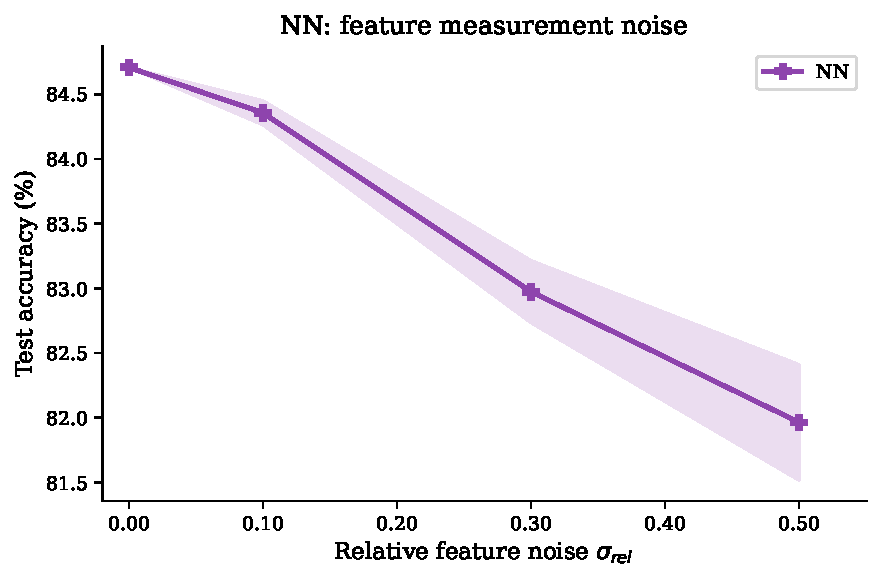
\includegraphics[width=0.7\textwidth]{img/usecase/feature_noise_accuracy.pdf}
\caption{Baseline \ac{NN} test accuracy as a function of relative feature noise $\sigma_{\text{rel}}$. Accuracy degrades monotonically from 84.7\% at $\sigma_{\text{rel}} = 0$ to 82.0\% at $\sigma_{\text{rel}} = 0.5$.}
\label{fig:feature_noise_accuracy}
\end{figure}

\begin{figure}[h]
\centering
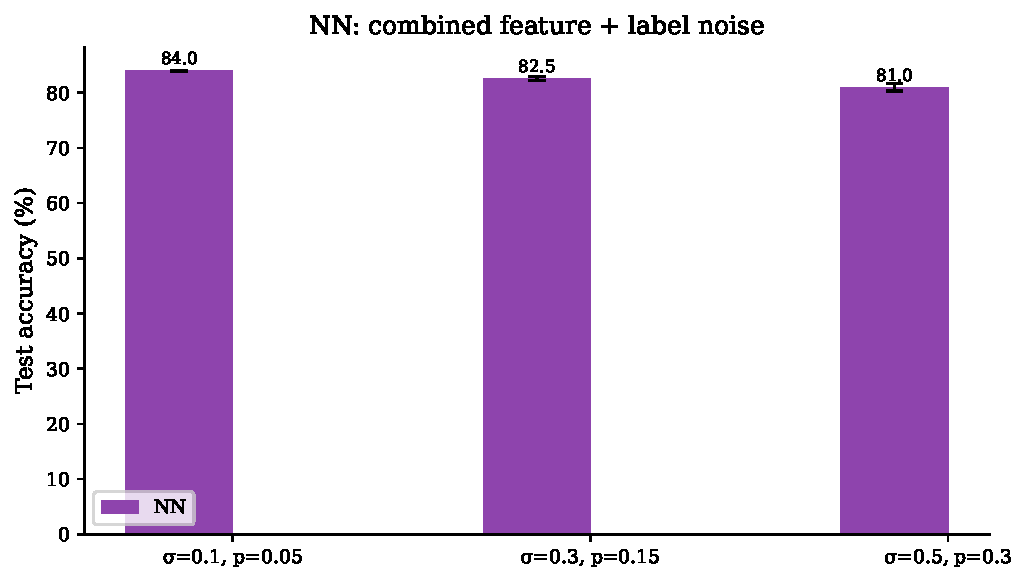
\includegraphics[width=0.7\textwidth]{img/usecase/combined_accuracy.pdf}
\caption{Baseline \ac{NN} test accuracy under combined feature and label noise. Accuracy degrades from 84.0\% at $(\sigma, p) = (0.1, 0.05)$ to 81.0\% at $(\sigma, p) = (0.5, 0.30)$.}
\label{fig:combined_accuracy}
\end{figure}

The \ac{NN} exhibits graceful degradation: accuracy decreases steadily but does not collapse, with a loss of 2.7 percentage points across the full feature-noise range and 3.0 percentage points across the combined-noise range. \Cref{fig:learning_curves} shows the corresponding learning curves over 10 training epochs. Convergence is stable across all conditions, confirming that the noise levels explored do not destabilize gradient-based learning.

\begin{figure}[h]
\centering
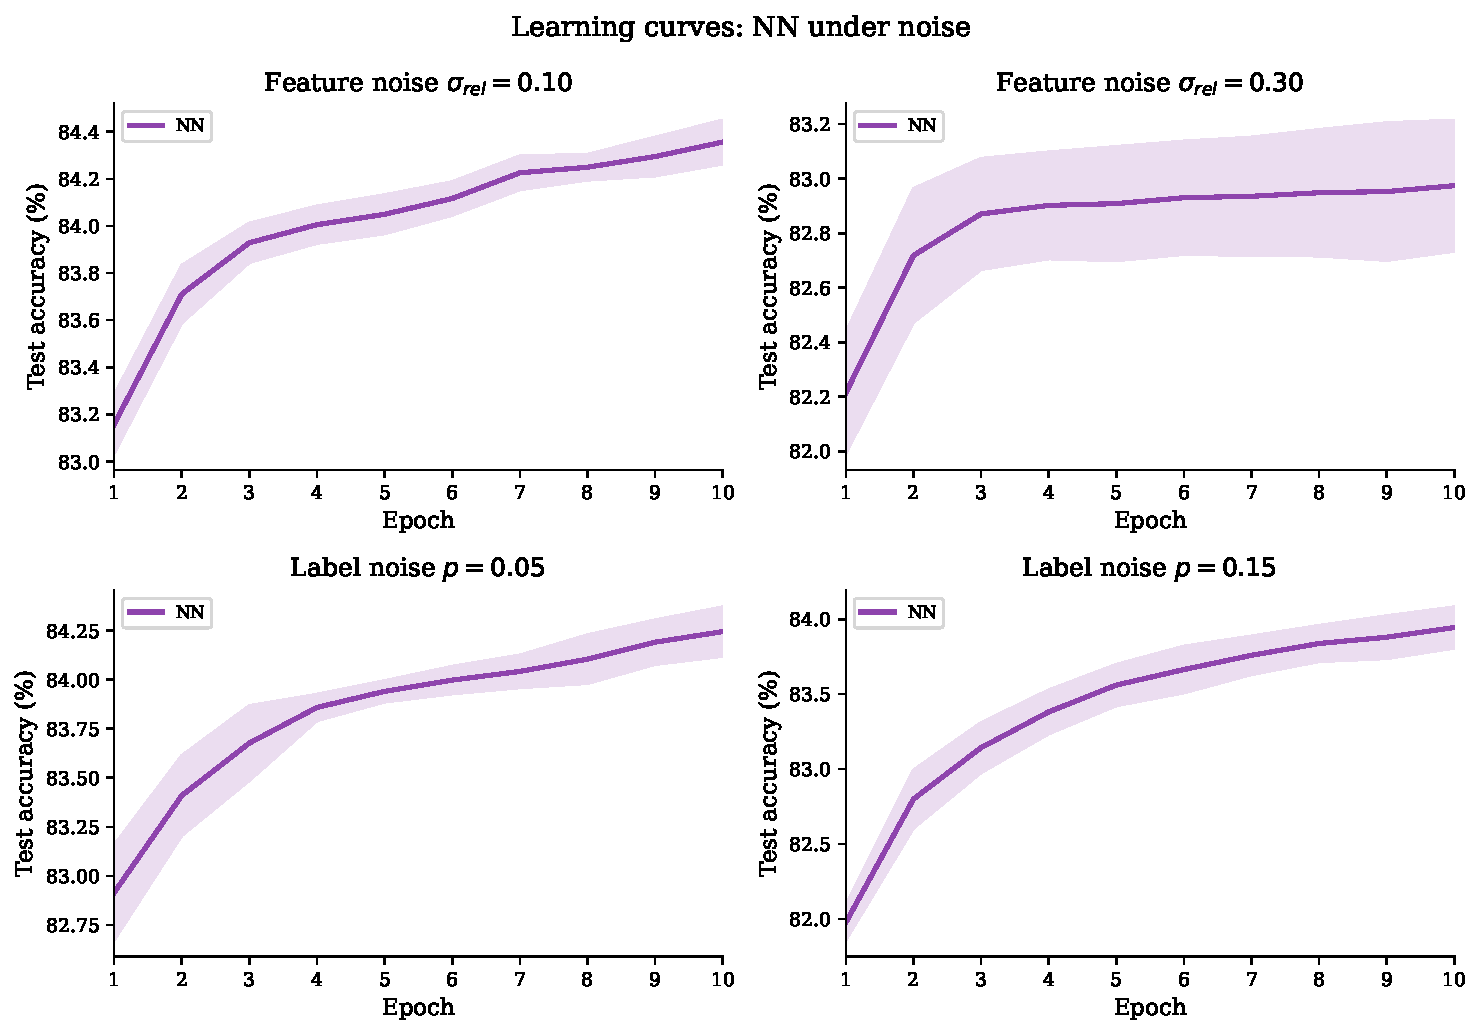
\includegraphics[width=\textwidth]{img/usecase/learning_curves.pdf}
\caption{Learning curves of the baseline \ac{NN} under feature noise ($\sigma_{\text{rel}} \in \{0.1, 0.3\}$, top) and label noise ($p \in \{0.05, 0.15\}$, bottom). All four conditions show monotonic convergence within 3 to 4 epochs, with final test accuracy between 82\% and 84\%.}
\label{fig:learning_curves}
\end{figure}


\subsection{Trust Opinion Mapping and Propagation Behavior}
\label{sec:trust_mapping_results}

Before evaluating the discriminative power of \ac{PaTAS} opinions, we verify that the calibration functions of \Cref{sec:trust_quantification} produce the expected mapping at the input layer. \Cref{fig:trust_mapping} visualizes the mapping for both noise sources, and \Cref{tab:trust-mapping} reports the numerical values used in our experiments.

\begin{figure}[h]
\centering
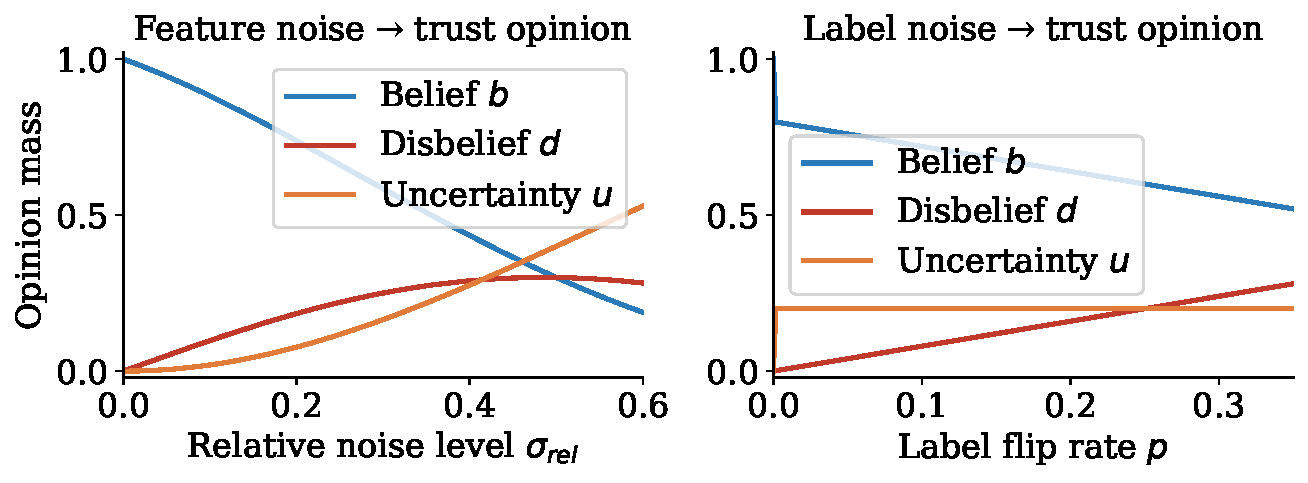
\includegraphics[width=\textwidth]{img/usecase/trust_mapping.pdf}
\caption{Trust opinion mapping at the input layer. Left: feature noise produces uncertainty-dominant opinions where $u$ grows with $\sigma_{\text{rel}}$ following \Cref{eq:feature_u}. Right: label noise produces disbelief-dominant opinions with $b = 1 - p$, $d = p$, and $u = 0$.}
\label{fig:trust_mapping}
\end{figure}

\input{img/usecase/trust_mapping}

The figure confirms the qualitatively distinct profiles designed into the two calibration functions. Feature noise produces increasing uncertainty, reaching $u = 0.40$ at $\sigma_{\text{rel}} = 0.5$ with correspondingly reduced belief and modest disbelief. Label noise produces a clean partition between belief and disbelief with zero residual uncertainty, consistent with the deterministic nature of the flip-rate model.

\paragraph{Propagation to the output layer.}
These input opinions are then propagated through the trained network for parameter trust quantification described in \Cref{sec:trust_propagation}. The benefit of this propagation is that the output opinion on each predicted class reflects both the quality of the input and the accumulated evidence about parameter reliability acquired during training. Because \ac{PaTAS} leaves the \ac{NN}'s predictions unchanged, the relevant evaluation question is not the magnitude of the output opinion in isolation, but whether it is informative about whether the prediction is correct. The following subsections answer this question directly.


\subsection{\ac{PaTAS} as a Discriminator of Correct Predictions}
\label{sec:patas_discriminator}

The central empirical question is whether \ac{PaTAS} opinions distinguish between correct and wrong \ac{NN} predictions. We compute the mean opinion components $(\bar{b}, \bar{d}, \bar{u})$ in the \ac{NN}'s predicted class, separately for samples where the prediction is correct and where it is wrong. A useful confidence signal should exhibit three simultaneous patterns:

\begin{itemize}
    \item Higher belief on correct predictions: $\bar{b}_c > \bar{b}_w$, i.e., $\Delta b > 0$.
    \item Lower uncertainty on correct predictions: $\bar{u}_c < \bar{u}_w$, i.e., $\Delta u < 0$.
    \item Lower disbelief on correct predictions: $\bar{d}_c < \bar{d}_w$, i.e., $\Delta d < 0$.
\end{itemize}

\Cref{fig:patas_effectiveness} visualizes these opinion masses, and \Cref{tab:ptas-effectiveness} reports the exact values.



% \begin{figure}[h]
% \centering
% 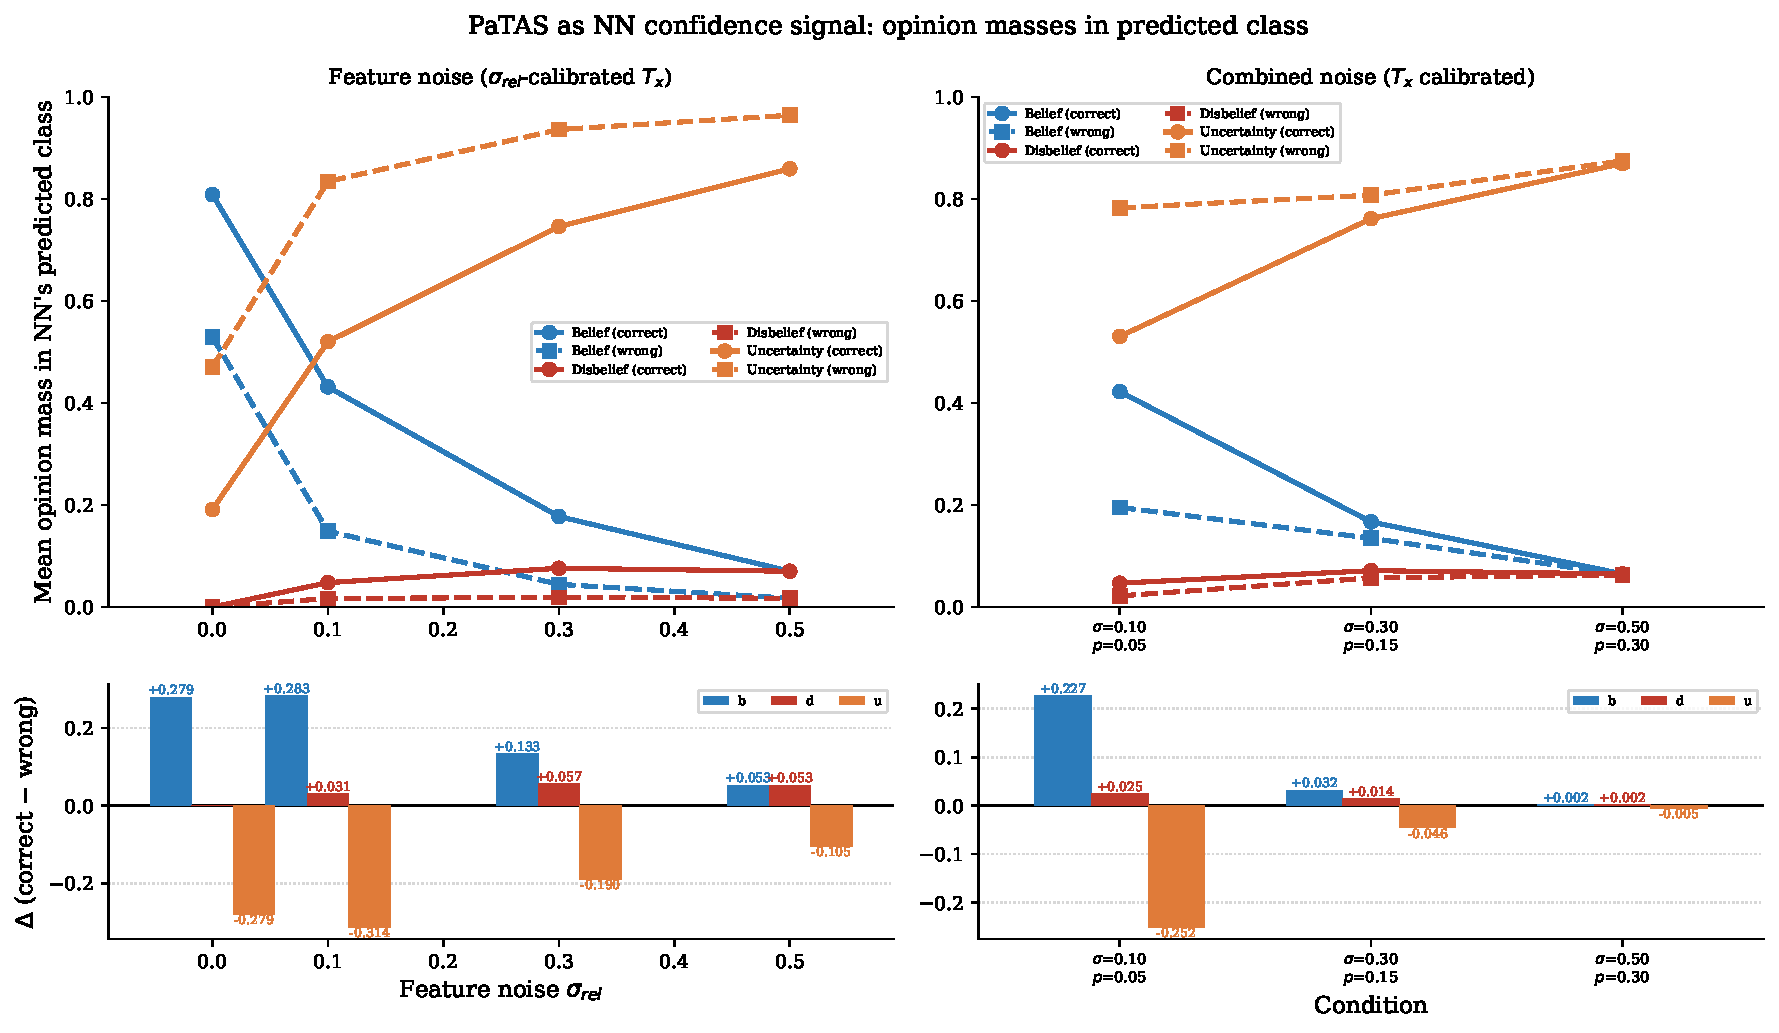
\includegraphics[width=\textwidth]{img/usecase/patas_effectiveness_test.pdf}
% \caption{\ac{PaTAS} opinion masses in the \ac{NN}'s predicted class. Top: mean opinion values for correctly-classified (solid lines, circles) versus mis-classified (dashed lines, squares) samples. Bottom: $\Delta = \text{correct} - \text{wrong}$, showing the discriminative gap per component. Left: feature noise. Right: combined noise.}
% \label{fig:patas_effectiveness}
% \end{figure}
\begin{figure}
    \centering
    \begin{subfigure}{0.7\textwidth}
        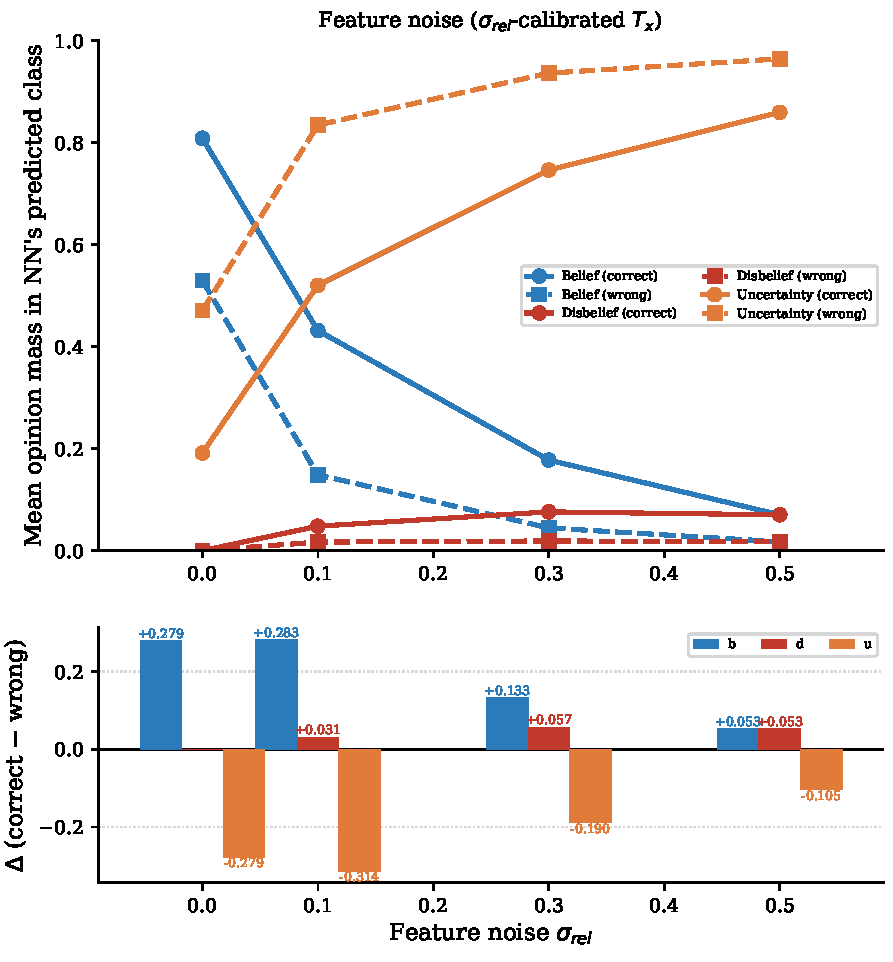
\includegraphics[width=\linewidth]{img/usecase/patas_effectiveness_test_cropped_1.pdf}
    \end{subfigure}
    \begin{subfigure}{0.7\textwidth}
        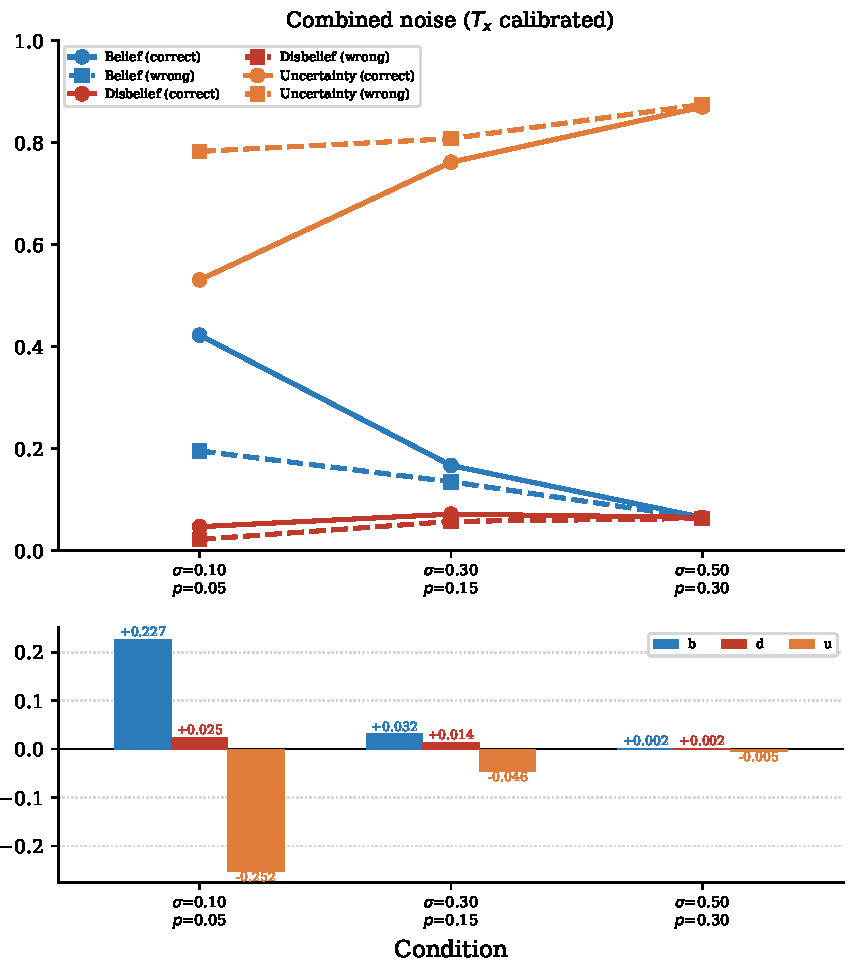
\includegraphics[width=\linewidth]{img/usecase/patas_effectiveness_test_cropped_2.pdf}
    \end{subfigure}
    \caption{\ac{PaTAS} opinion masses in the \ac{NN}'s predicted class. Top: mean opinion values for correctly-classified (solid lines, circles) versus mis-classified (dashed lines, squares) samples. Bottom: $\Delta = \text{correct} - \text{wrong}$, showing the discriminative gap per component. Left: feature noise. Right: combined noise.}
\label{fig:patas_effectiveness}
\end{figure}

\begin{table}[ht]
\centering
\caption{Mean \ac{PaTAS} opinion masses $(b, d, u)$ in the \ac{NN}'s predicted class, split by correct ($c$) vs.\ wrong ($w$) NN predictions. $\Delta = \text{correct} - \text{wrong}$; positive $\Delta b$ and negative $\Delta d$/$\Delta u$ indicate discriminability.}
\label{tab:ptas-effectiveness}
\begin{tabular}{lccccccccccc}
\toprule
Noise & $N_c$ & $N_w$ & $\bar{b}_c$ & $\bar{b}_w$ & $\Delta b$ & $\bar{d}_c$ & $\bar{d}_w$ & $\Delta d$ & $\bar{u}_c$ & $\bar{u}_w$ & $\Delta u$ \\
\hline
Feature noise \\
0.00 & 15692 & 2833 & 0.81 & 0.53 & +0.28 & 0.00 & -0.00 & +0.00 & 0.19 & 0.47 & -0.28 \\
0.10 & 15608 & 2917 & 0.43 & 0.15 & +0.28 & 0.05 & 0.02 & +0.03 & 0.52 & 0.83 & -0.31 \\
0.30 & 15407 & 3118 & 0.18 & 0.04 & +0.13 & 0.08 & 0.02 & +0.06 & 0.75 & 0.94 & -0.19\\
0.50 & 15265 & 3260 & 0.07 & 0.02 & +0.05 & 0.07 & 0.02 & +0.05 & 0.86 & 0.96 & -0.11 \\
\hline 
Combined noise \\
(0.10, 0.05) & 15527 & 2998 & 0.42 & 0.20 & +0.23 & 0.05 & 0.02 & +0.03 & 0.53 & 0.78 & -0.25 \\
(0.30, 0.15) & 15333 & 3192 & 0.17 & 0.14 & +0.03 & 0.07 & 0.06 & +0.01 & 0.76 & 0.81 & -0.05 \\
(0.50, 0.30) & 15061 & 3464 & 0.07 & 0.06 & +0.01 & 0.07 & 0.06 & +0.01 & 0.87 & 0.87 & -0.01 \\
\bottomrule
\end{tabular}
\end{table}

The results confirm clear discriminability under moderate noise:

\begin{itemize}
    \item At $\sigma_{\text{rel}} = 0.10$, \ac{PaTAS} belief on correct predictions ($\bar{b}_c = 0.43$) is nearly three times higher than on wrong predictions ($\bar{b}_w = 0.15$), yielding $\Delta b = +0.28$. Uncertainty exhibits the opposite pattern ($\Delta u = -0.31$), while disbelief remains low across both groups ($\bar{d} < 0.05$), confirming that \ac{PaTAS} treats feature noise as epistemic uncertainty rather than evidence of deception.
    \item At $\sigma_{\text{rel}} = 0.30$, discriminability persists but narrows ($\Delta b = +0.13$, $\Delta u = -0.19$), reflecting the degraded quality of the input trust signal as noise increases.
    \item At $\sigma_{\text{rel}} = 0.50$, both correct and wrong predictions receive similar opinions ($\Delta b = +0.05$). This is the expected behavior: when input quality approaches the maximum noise level, \ac{PaTAS} correctly signals that no prediction can be trusted, and the discriminative gap collapses accordingly.
\end{itemize}

Under combined noise, the discriminative gap at low corruption levels ($(\sigma, p) = (0.10, 0.05)$: $\Delta b = +0.23$) is comparable to the feature-only case, but narrows more sharply as both sources intensify together. At the most severe condition $(\sigma, p) = (0.50, 0.30)$, the gap is minimal ($\Delta b = +0.002$), with elevated uncertainty dominating both groups. This is consistent with the additive degradation of two independent noise sources simultaneously reducing the reliability of both input and label evidence available to the trust propagation mechanism.


\subsection{Selective Prediction Using \ac{PaTAS}}
\label{sec:selective_prediction}

A direct application of the discriminative capacity demonstrated above is selective prediction: rejecting predictions where the trust signal indicates low reliability, thereby improving accuracy on the retained subset. We evaluate two filters:

\begin{itemize}
    \item \textbf{\ac{PaTAS} filter} ($b > u$): retain samples where belief exceeds uncertainty in the predicted class, indicating that positive evidence for the prediction outweighs residual epistemic doubt.
    \item \textbf{Softmax filter} ($\text{softmax} > 0.5$): retain samples where the \ac{NN} softmax probability in the predicted class exceeds 0.5, the standard high-confidence threshold.
\end{itemize}

\Cref{tab:threshold-b-gt-d,tab:threshold-nn-0-50} compare the two filters across noise conditions.

\begin{table}[ht]
\centering
\caption{Selective prediction: \ac{PaTAS} belief-over-uncertainty filter ($b > u$). Coverage is the fraction of test samples where \ac{PaTAS} belief exceeds uncetainty in the \ac{NN}'s predicted class (net positive subjective evidence). Values are mean $\pm$ std over 5 independent runs.}
\label{tab:threshold-b-gt-d}
\begin{tabular}{lccc}
\toprule
Noise condition & Coverage (\%) & Accuracy on covered (\%) & Overall accuracy (\%) \\
\hline
\multicolumn{4}{l}{\textit{Feature noise ($T_x$ calibrated to $\sigma_{rel}$)}} \\
$\sigma_{rel}=0.10$ & 49.6 $\pm$ 16.5 & 89.38 $\pm$ 1.26 & 84.33 \\
\hline
\multicolumn{4}{l}{\textit{Combined noise ($T_x$ calibrated to $\sigma_{rel}$)}} \\
$\sigma=0.10,\,p=0.05$ & 32.7 $\pm$ 0.2 & 89.40 $\pm$ 2.23 & 84.00 \\
\bottomrule
\end{tabular}
\end{table}


\begin{table}[ht]
\centering
\caption{Selective prediction: NN softmax score threshold $\tau = 0.5$. Coverage is the fraction of test samples where the NN softmax probability in the predicted class exceeds $0.5$. Values are mean $\pm$ std over 5 independent runs.}
\label{tab:threshold-nn-0-50}
\begin{tabular}{lccc}
\toprule
Noise condition & Coverage (\%) & Accuracy on covered (\%) & Overall accuracy (\%) \\
\midrule
\multicolumn{4}{l}{\textit{Feature noise ($T_x$ calibrated to $\sigma_{rel}$)}} \\
$\sigma_{rel}=0.10$ & 97.9 $\pm$ 0.2 & 85.15 $\pm$ 0.09 & 84.36 \\
\midrule 
\multicolumn{4}{l}{\textit{Combined noise ($T_x$ calibrated to $\sigma_{rel}$)}} \\
$\sigma=0.10,\,p=0.05$ & 95.4 $\pm$ 0.3 & 85.73 $\pm$ 0.17 & 84.01 \\
\bottomrule
\end{tabular}
\end{table}


The \ac{PaTAS} filter is more selective and more accurate than the softmax filter across all evaluated conditions:

\begin{itemize}
    \item At $\sigma_{\text{rel}} = 0.10$, the \ac{PaTAS} filter retains 49.6\% of samples and achieves 89.4\% accuracy on that subset, a gain of 5.0 percentage points over the overall accuracy of 84.4\%. The softmax filter retains 97.9\% of samples but improves accuracy by only 0.8 percentage points (from 84.4\% to 85.2\%).
    \item Under combined noise at $(\sigma, p) = (0.10, 0.05)$, the \ac{PaTAS} filter achieves 89.4\% accuracy on 32.7\% coverage, while softmax achieves 85.7\% on 95.4\% coverage.
    \item The accuracy advantage of \ac{PaTAS} over softmax narrows as noise increases, consistent with the decreasing discriminative gap observed in \Cref{sec:patas_discriminator}.
\end{itemize}

The higher selectivity of the \ac{PaTAS} filter comes at the cost of coverage: at $\sigma_{\text{rel}} = 0.10$, half the samples are rejected. This trade-off is inherent to any threshold-based filter and depends on the deployment context. In high-stakes settings where incorrect predictions carry a high cost, the \ac{PaTAS} filter's precision is preferable. In settings where coverage matters, the two signals can be combined: samples passing the \ac{PaTAS} filter receive the trust-based accuracy guarantee, while remaining samples can be handled by a fallback strategy or flagged for human review.


\subsection{Summary of Robustness Findings}
\label{sec:robustness_summary}

Three conclusions follow from the empirical results:

\begin{enumerate}
    \item \ac{PaTAS} belief discriminates between correct and wrong predictions across all evaluated noise conditions. The discriminative gap $\Delta b$ ranges from $+0.28$ at low feature noise to $+0.05$ at high noise, with graceful degradation as data quality deteriorates.
    \item The nature of discrimination is consistent with the trust calibration design: feature noise produces uncertainty-driven separation ($\Delta u$ is the dominant signal), while combined noise produces a mixed signal with both uncertainty and belief components contributing.
    \item Used as a selective prediction filter, \ac{PaTAS} improves accuracy by 5.0 to 5.6 percentage points on retained samples, compared to 0.8 to 1.7 for softmax thresholding. The advantage derives from two complementary properties. First, the three-component opinion $(b, d, u)$ distinguishes vacuous predictions (high $u$, low $b$) from genuinely confident ones in a way that a single softmax probability cannot. Second, and more fundamentally, the trust opinion encodes explicit knowledge of data quality: the noise level $\sigma_i$ of each training sample is mapped to a calibrated opinion via $\text{feature\_noise\_to\_trust}(\sigma_i)$, and this quality signal propagates through the Trust Nodes Network alongside the standard forward pass. The output opinion therefore reflects not only the network's learned confidence but also how reliable the data used to form that confidence actually was. Softmax probabilities have no access to this provenance information and treat all predictions as equally grounded in the training data.
\end{enumerate}

\section{Calibration Quantification using Subjective Logic}
\label{sec:calibration_quantification}

The previous section evaluated PaTAS as a per-prediction confidence signal. We now turn to a complementary question: \emph{can we produce a single trust opinion that characterizes the trustworthiness of an entire trained model?} This is the calibration-trust problem, which we addressed in our earlier work using \acf{BPQ} with cumulative fusion across probability clusters (\cref{chap:bb}).

Unlike PaTAS, calibration quantification operates post-hoc on the predictions of an already-trained NN. The two methods are complementary: PaTAS provides per-sample trust during inference; calibration quantification provides a global trust opinion on the model itself. Evaluating both under the same noise conditions allows us to capture different aspects of trustworthiness.


\subsection{Methodology Recap}
\label{sec:calibration_methodology}

The calibration-trust algorithm (\cref{alg:1} in \cref{chap:bb}) computes a single binomial opinion $(b, d, u)$ on the trained NN as follows:
\begin{enumerate}
    \item \textbf{Clustering predictions.} The predicted probabilities for each class are partitioned into $M = 10$ bins over $[0, 1]$.
    \item \textbf{Per-cluster evidence.} For each bin $i$ with representative probability $\text{RP}_i$, positive evidence is the number of correct classifications $t_i$, and negative evidence is $|t_i - n_i \cdot \text{RP}_i|$, measuring the deviation between predicted and observed accuracy.
    \item \textbf{Per-cluster opinion.} A binomial opinion is computed via BPQ with uncertainty weight $W = 2$.
    \item \textbf{Cumulative fusion.} Cluster opinions are fused per class, then across classes, yielding a single calibration-trust opinion for the NN.
\end{enumerate}

This procedure quantifies how well the model's predicted probabilities align with its actual accuracy: a perfectly calibrated model receives an opinion approaching $(1, 0, 0)$, while a miscalibrated model shows elevated disbelief.


\subsection{Calibration Trust Across Noise Conditions}
\label{sec:calibration_results}
We compute calibration trust for the same trained networks evaluated in \Cref{sec:noise_robustness}, under feature noise, label noise, and combined noise. \Cref{fig:calibration_trust} visualizes the resulting opinion masses, and \Cref{tab:calibration-trust} reports the numerical values.

\begin{figure}[h]
\centering
% 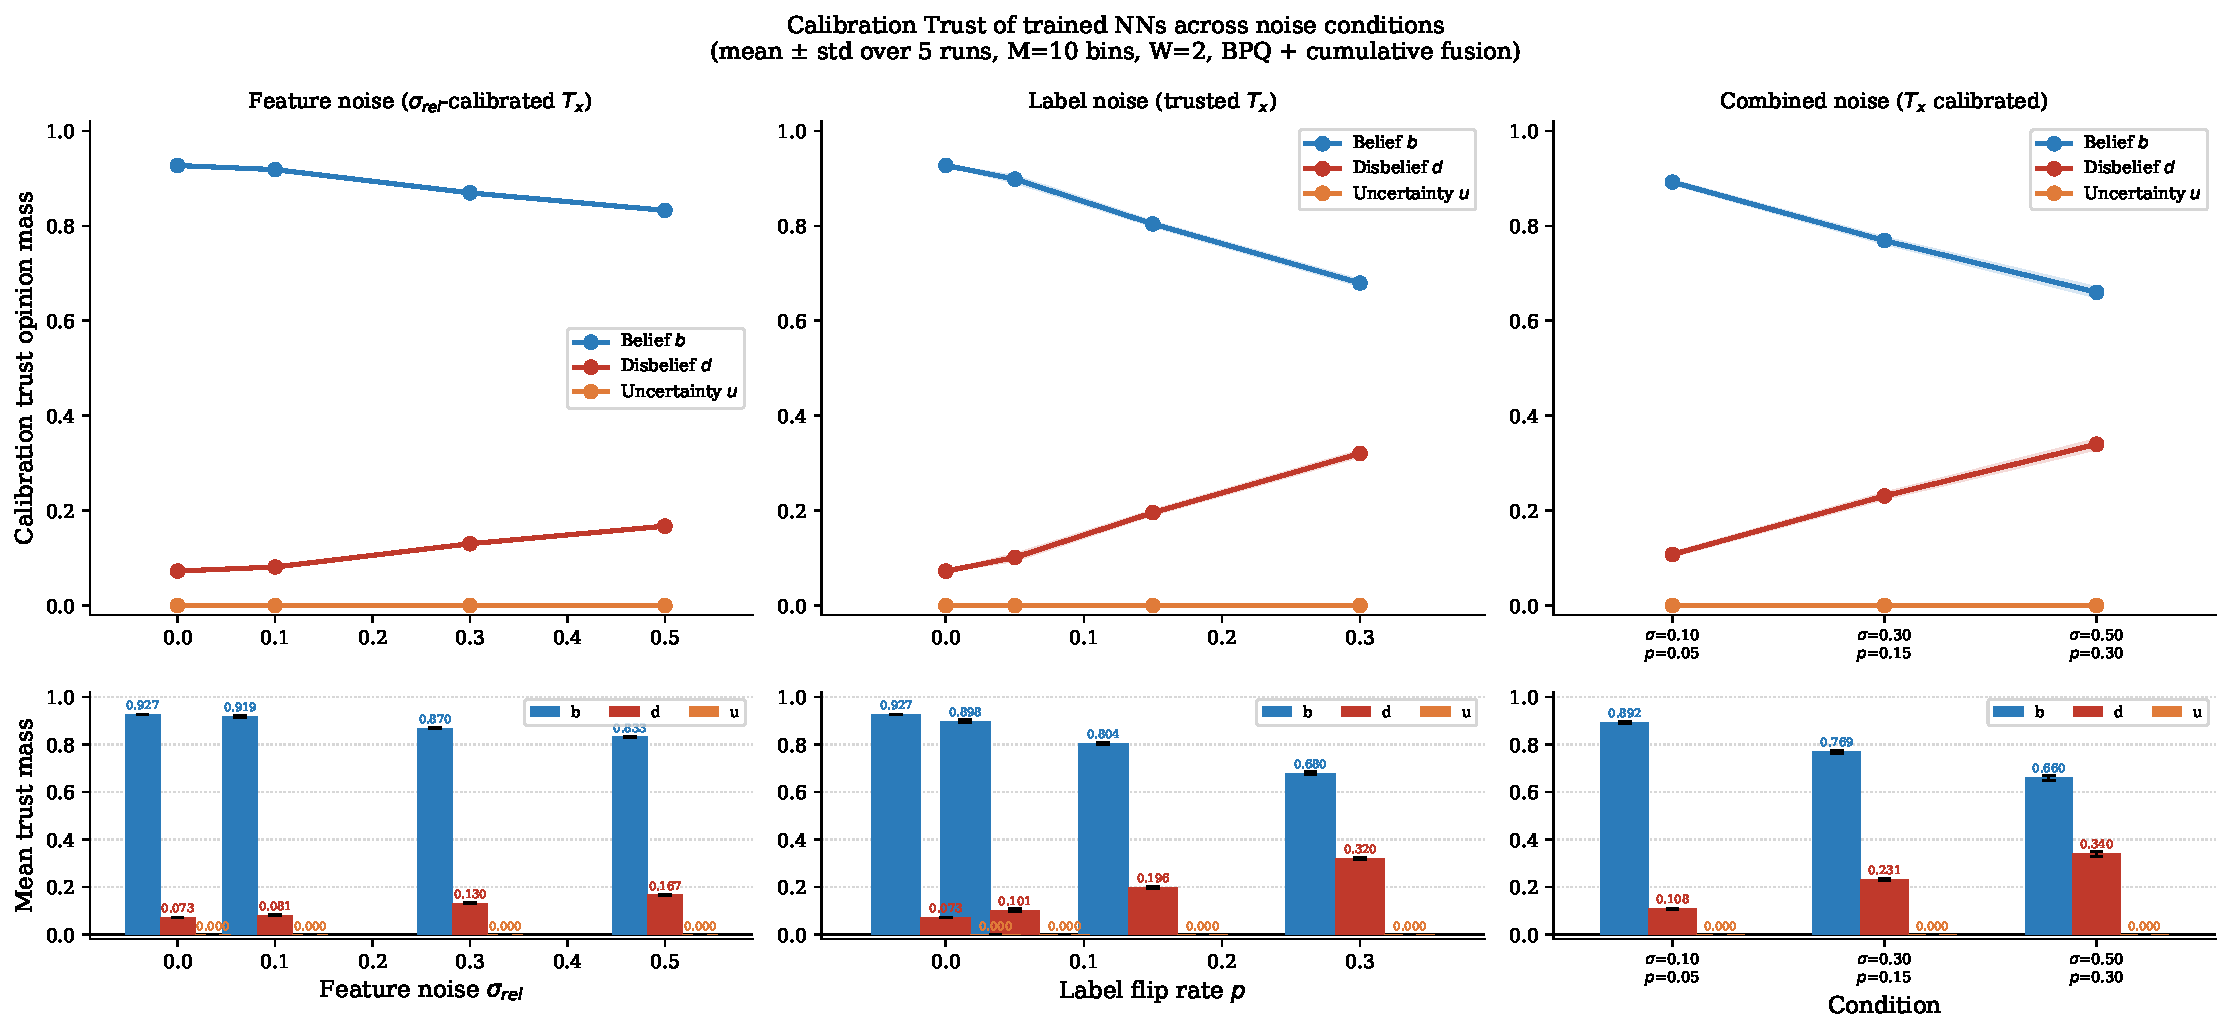
\includegraphics[width=\textwidth]{img/usecase/calibration_trust.pdf}
\begin{subfigure}{0.49\textwidth}
    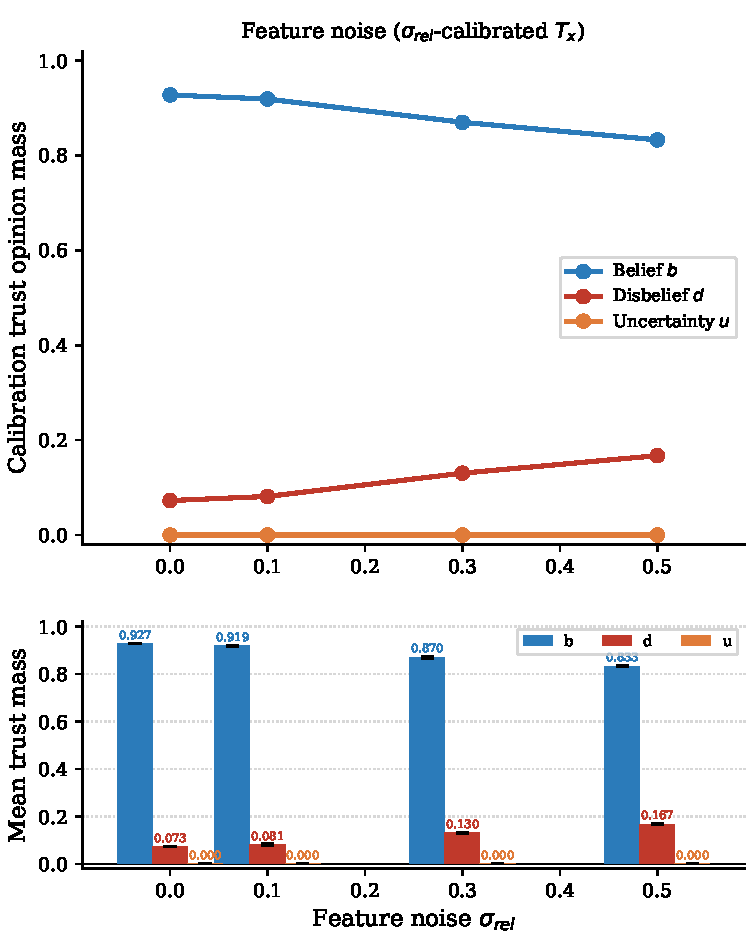
\includegraphics[width=\textwidth]{img/usecase/calibration_trust_cropped_1.pdf}
\end{subfigure}
\begin{subfigure}{0.49\textwidth}
    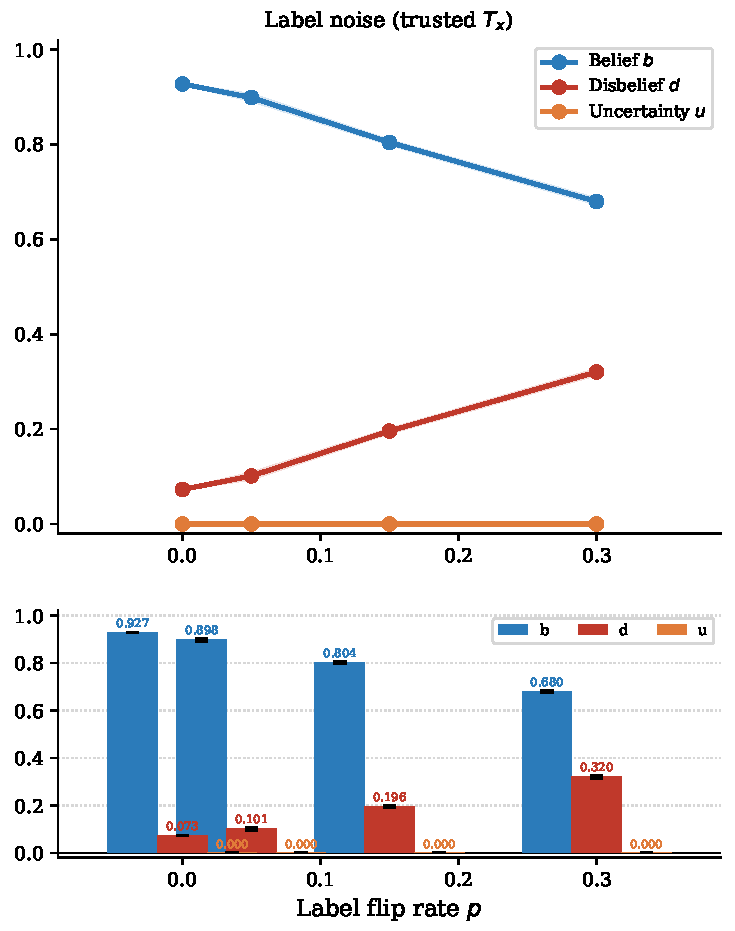
\includegraphics[width=\textwidth]{img/usecase/calibration_trust_cropped_2.pdf}
\end{subfigure}
\begin{subfigure}{0.49\textwidth}
    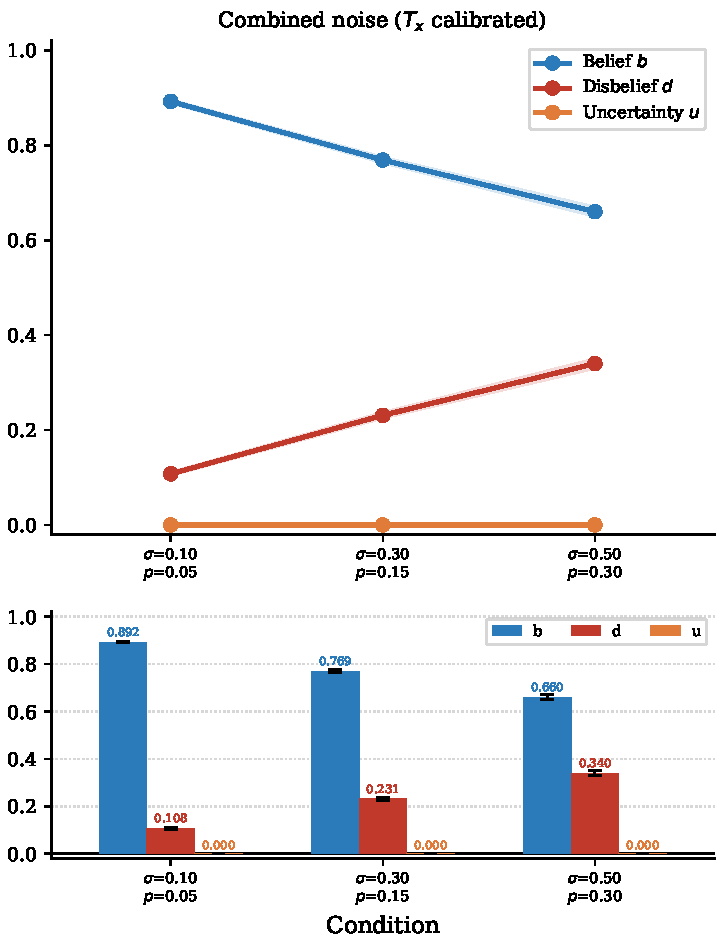
\includegraphics[width=\textwidth]{img/usecase/calibration_trust_cropped_3.pdf}
\end{subfigure}
\caption{Calibration trust of trained NNs across noise conditions, computed via BPQ with cumulative fusion ($M = 10$ bins, $W = 2$). Top: opinion masses as a function of noise magnitude. Bottom: numerical values per condition. Left: feature noise. Center: label noise. Right: combined noise. Mean $\pm$ standard deviation over 5 independent runs.}
\label{fig:calibration_trust}
\end{figure}

\begin{table}[ht]
\centering
\caption{calibration-trust opinions for trained NNs across noise conditions. Opinions averaged over 5 independent runs. High belief $b$ indicates a well-calibrated, trustworthy model; high uncertainty $u$ indicates insufficient evidence.}
\label{tab:calibration-trust}
\begin{tabular}{lcccc}
\toprule
Condition & Belief $b$ (mean$\pm$std) & Disbelief $d$ (mean$\pm$std) & Uncertainty $u$ (mean$\pm$std)\\
\hline
Feature noise \\
0.00 & 0.93$\pm$0.00 & 0.07$\pm$0.00 & 0.01$\pm$0.00 \\
0.10 & 0.93$\pm$0.01 & 0.08$\pm$0.01 & 0.01$\pm$0.01 \\
0.30 & 0.87$\pm$0.01 & 0.13$\pm$0.01 & 0.01$\pm$0.00 \\
0.50 & 0.83$\pm$0.01 & 0.17$\pm$0.01 & 0.01$\pm$0.00 \\
\hline 
Label noise  \\
0.00 & 0.93$\pm$0.00 & 0.07$\pm$0.00 & 0.01$\pm$0.00 \\
0.05 & 0.90$\pm$0.01 & 0.10$\pm$0.01 & 0.01$\pm$0.00 \\
0.15 & 0.80$\pm$0.01 & 0.20$\pm$0.01 & 0.01$\pm$0.00 \\
0.30 & 0.68$\pm$0.02 & 0.32$\pm$0.01 & 0.01$\pm$0.00\\
\hline
Combined noise \\
(0.10,0.05) & 0.89$\pm$0.01 & 0.11$\pm$0.01 & 0.01$\pm$0.00 \\
(0.30,0.15) & 0.77$\pm$0.01 & 0.23$\pm$0.01 & 0.01$\pm$0.00  \\
(0.50,0.30) & 0.66$\pm$0.01 & 0.34$\pm$0.01 & 0.01$\pm$0.00 \\
\bottomrule
\end{tabular}
\end{table}

\paragraph{Feature noise has limited impact on calibration.}
As $\sigma_{\text{rel}}$ increases from $0$ to $0.5$, belief decreases only modestly from $0.927$ to $0.833$, while disbelief rises from $0.073$ to $0.167$. The model remains well-calibrated despite degraded inputs, indicating that its confidence values continue to track empirical accuracy even when the underlying data is noisier. This is consistent with the graceful accuracy degradation seen in \Cref{sec:baseline_nn}. \todo{Add also that noise adding is a differential privacy\cite{} way to avoid overconfidence. so noise is not so bad}

\paragraph{Label noise causes substantial miscalibration.}
Label flipping has a much stronger effect: at $p = 0.30$, belief drops to $0.680$ and disbelief rises to $0.320$. When training labels are systematically wrong, the model learns to be confident in incorrect predictions, breaking the alignment between predicted probabilities and true accuracy. Calibration trust correctly identifies this as the more severe form of corruption.

\paragraph{Combined noise compounds the effect.}
Under combined corruption, calibration trust degrades faster than under either source alone. At $(\sigma, p) = (0.50, 0.30)$, belief falls to $0.660$, the lowest across all conditions. The dominant driver is label noise, with feature noise contributing additively but secondarily.

\paragraph{Uncertainty remains negligible.}
Across all conditions, uncertainty $u$ stays near $10^{-4}$. With a large test set (over 18{,}000 samples distributed across $M = 10$ bins and 3 classes), the evidence weight $W = 2$ becomes negligible relative to the cumulative evidence, driving $u \to 0$. The opinion collapses toward a Beta distribution with well-determined belief and disbelief, leaving little residual uncertainty.


\subsection{Comparison: Per-Prediction Trust vs.\ Calibration Trust}
\label{sec:patas_vs_calibration}

PaTAS opinions and calibration-trust opinions answer different questions about the same trained network. \Cref{tab:trust_comparison} summarizes the distinction.

\begin{table}[h]
\centering
\caption{Per-prediction trust (PaTAS) versus global calibration trust.}
\label{tab:trust_comparison}
\begin{tabular}{lll}
\toprule
Aspect & PaTAS (per-prediction) & Calibration trust (global) \\
\midrule
Granularity & One opinion per sample & One opinion per model \\
Computation & Forward through \ac{TNN} & Post-hoc on predictions \\
Dominant component & Uncertainty (feature noise) & Dis/belief (miscalibration) \\
Use case & Selective prediction & Model auditing \\
% Signal at high noise & Degrades to vacuous & Degrades to high disbelief \\
\bottomrule
\end{tabular}
\end{table}

The two methods complement each other. PaTAS opinions express \emph{uncertainty about a specific prediction} given the input quality: a high-uncertainty PaTAS opinion suggests the input itself is unreliable. Calibration-trust opinions express \emph{belief/disbelief in the model's confidence calibration} given its observed accuracy: a high-disbelief or low belief calibration opinion suggests the model is miscalibrated and its confidence values cannot be trusted. Used together, the two trust assessments provide a comprehensive picture: PaTAS identifies which predictions to trust at inference time; calibration trust assesses whether to trust the model as a whole in terms of score predicted.


\section{Discussion}
\label{sec:discussion}


\subsection{What PaTAS Adds Beyond Softmax Confidence}
\label{sec:discussion_softmax}

Softmax probabilities collapse confidence into a single number, while PaTAS produces a three-component opinion $(b, d, u)$. This distinction is meaningful for several reasons:

\begin{itemize}
    \item \textbf{Uncertainty separation.} PaTAS distinguishes between low confidence due to insufficient evidence (high $u$, low $d$) and low confidence due to conflicting evidence (low $u$, high $d$). Softmax conflates these into a single low-probability output.
    \item \textbf{Traceable origins.} Because PaTAS opinions are constructed by propagating input opinions through the network, uncertainty in a prediction can be traced back to specific noisy inputs or unreliable parameters.
    \item \textbf{Operational interpretation.} The components $(b, d, u)$ map to distinct decisions: high $u$ suggests collecting more data; high $d$ suggests auditing the labeling process.
\end{itemize}


\subsection{Computational Cost}
\label{sec:computational_cost}

We measured the latency overhead of running PaTAS alongside the standard neural network, both at inference and during training. The results are summarized in \Cref{fig:patas_latency}, with detailed numbers in \Cref{tab:latency-inference,tab:latency-training}.

\begin{figure}[h]
\centering
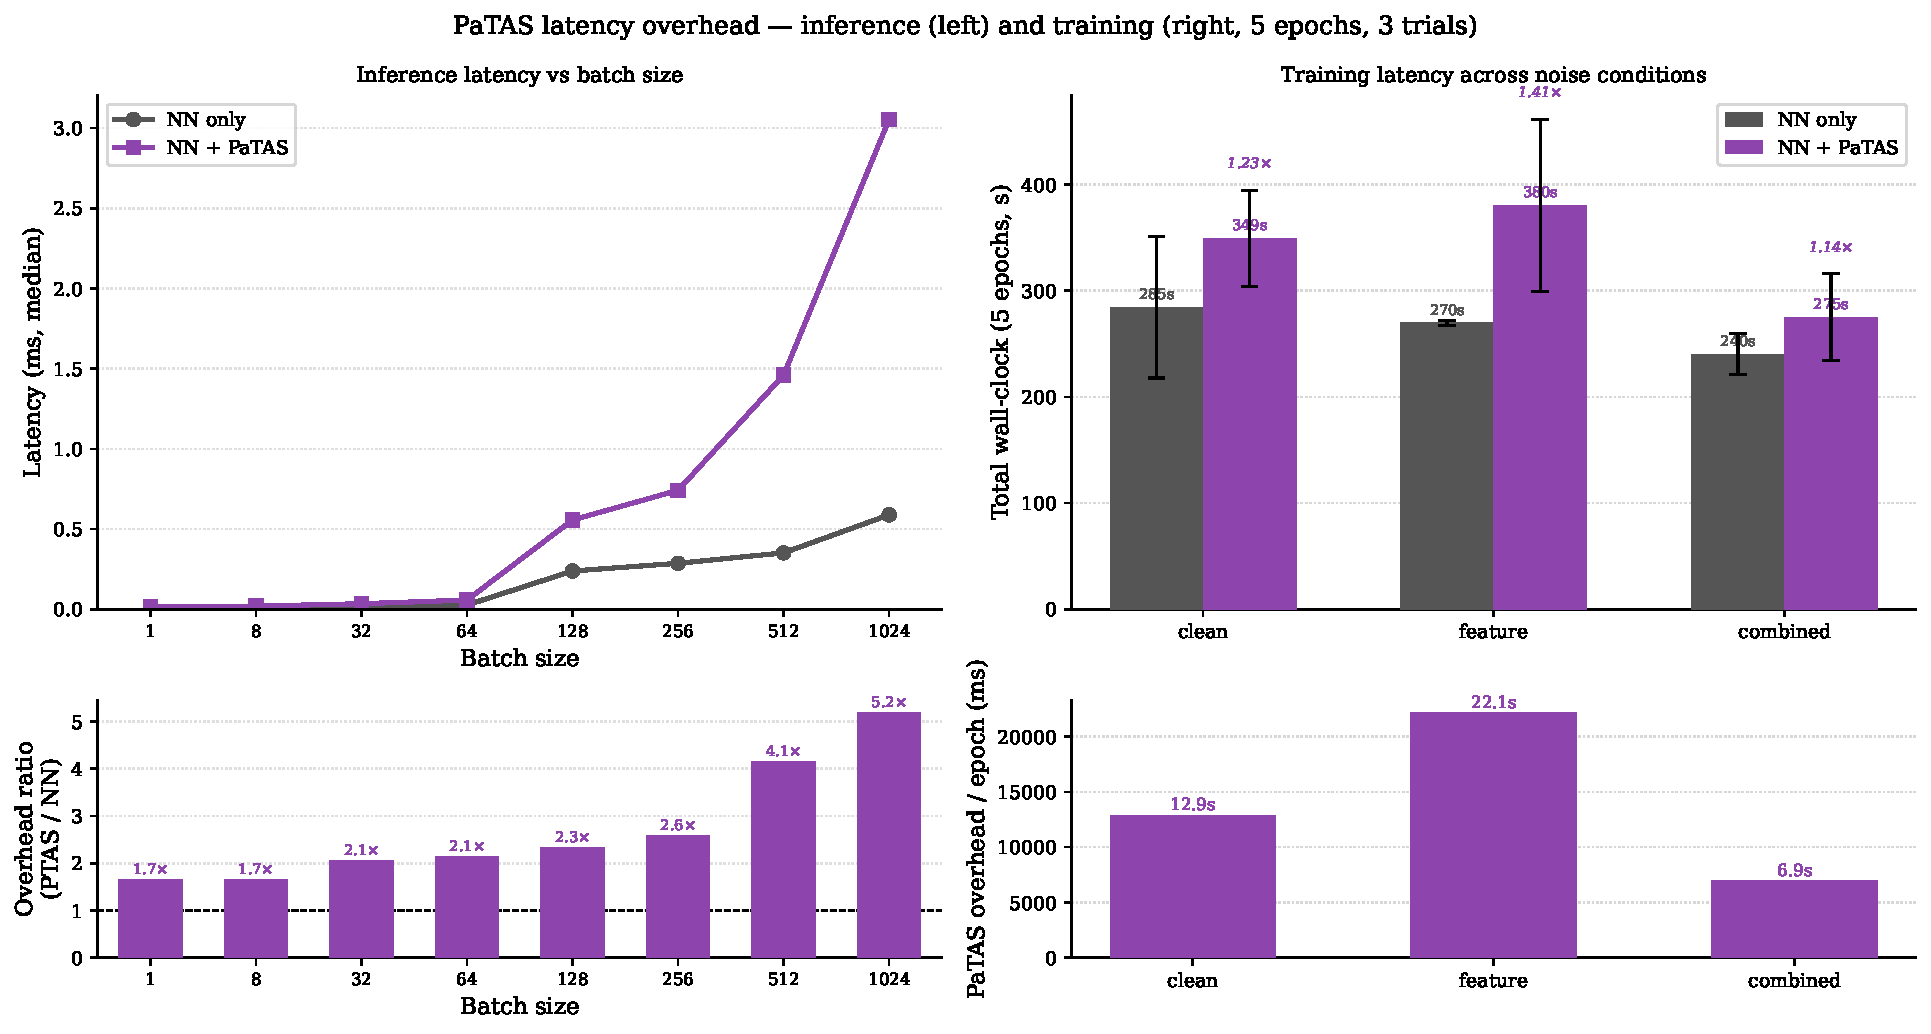
\includegraphics[width=\textwidth]{img/usecase/latency_plot.pdf}
\caption{PaTAS latency overhead. Left column: inference latency as a function of batch size; the upper plot shows absolute median latency (200 repetitions), the lower plot shows the PaTAS-to-NN overhead ratio. Right column: training wall-clock across noise conditions (mean $\pm$ std over 3 trials, 5 epochs each); the upper plot shows total time, the lower plot shows the per-epoch PaTAS overhead in milliseconds.}
\label{fig:patas_latency}
\end{figure}



\begin{table}[ht]
\centering
\caption{Training latency (mean $\pm$ std over 3 trials, 5 epochs) for plain NN vs PaTAS-augmented NN training. Overhead / epoch = per-epoch wall-clock difference.}
\label{tab:latency-training}
\begin{tabular}{lcccccc}
\toprule
Condition & NN tot(s) & PaTAS tot(s) & NN/ep(s) & PaTAS/ep(s) & Overhead/ep(ms) & Ratio($\times$) \\
\midrule
clean & 284.6$\pm$66.8 & 348.9$\pm$45.3 & 56.91 & 69.79 & 12874 & 1.23 \\
feature & 269.7$\pm$2.4 & 380.4$\pm$80.8 & 53.93 & 76.08 & 22144 & 1.41 \\
combined & 240.2$\pm$19.5 & 275.0$\pm$40.9 & 48.05 & 54.99 & 6944 & 1.14 \\
\bottomrule
\end{tabular}
\end{table}


\begin{table}[ht]
\centering
\caption{Inference latency (median over 200 repetitions) for plain NN forward pass vs PaTAS \texttt{apply\_feedforward}. Overhead ratio = PaTAS / NN.}
\label{tab:latency-inference}
\begin{tabular}{lccc}
\toprule
Batch size & NN latency (ms) & PaTAS latency (ms) & Overhead ratio ($\times$) \\
\midrule
1 & 0.009 & 0.015 & 1.66 \\
8 & 0.012 & 0.02 & 1.794 \\
32 & 0.017 & 0.035 & 2.044 \\
64 & 0.027 & 0.058 & 2.156 \\
128 & 0.239 & 0.557 & 2.330 \\
256 & 0.287 & 0.742 & 2.585 \\
512 & 0.352 & 1.460 & 4.15 \\
1024 & 0.589 & 3.054 & 5.189 \\
\bottomrule
\end{tabular}
\end{table}





\paragraph{Inference latency.}
At small batch sizes ($\leq 64$), PaTAS adds an absolute overhead of well under 0.1\,ms, with the relative overhead ratio between 1.7$\times$ and 2.2$\times$. At these sizes, both the NN forward pass and the trust feedforward through the Trust Nodes Network are dominated by per-call constants rather than by the size of the batch. As batch size grows, the overhead ratio increases more steeply: 2.6$\times$ at batch 256, 4.1$\times$ at batch 512, and 5.2$\times$ at batch 1024. In absolute terms, PaTAS adds roughly 2.5\,ms per inference at batch size 1024 (3.05\,ms total versus 0.59\,ms for the NN alone). This scaling reflects the fact that the trust discounting operator applied at each Trust Node performs more work per sample than a standard matrix multiplication: each sample carries a $(b, d, u)$ triple that must be discounted by the weight opinion at every neuron, accumulated, and combined across inputs.


\paragraph{Training overhead.}
Training overhead is more moderate than the inference overhead suggests, because the trust update step runs in parallel with the NN's backward pass over the TCP socket rather than blocking it. Over 5 epochs and 3 trials, total training time increased by 1.14$\times$ to 1.41$\times$ depending on the noise condition: 1.23$\times$ on clean data (285\,s $\to$ 349\,s), 1.41$\times$ under feature noise (270\,s $\to$ 380\,s), and 1.14$\times$ under combined noise (240\,s $\to$ 275\,s). The per-epoch overhead ranges from 6.9\,s to 22.1\,s. The variability across conditions (especially the high standard deviation on the clean and feature settings) reflects the TCP-based client-server architecture: trust message exchange is sensitive to scheduling, socket buffering, and process contention, all of which contribute additional jitter.


\paragraph{Implications for deployment.}
Three implications follow:

\begin{itemize}
    \item \textbf{Inference cost is acceptable for moderate batch sizes.} At batch sizes typical of streaming inference ($\leq 64$), the absolute overhead is sub-millisecond, well within typical service-level budgets. PaTAS is therefore practical for per-sample or small-batch deployment, which is the regime in which its per-prediction trust signal is most useful.
    \item \textbf{Large-batch inference incurs proportionally higher cost.} The 5.2$\times$ overhead at batch 1024 suggests that batched offline scoring with PaTAS should be reserved for cases where the trust signal is genuinely needed (for instance, periodic audits or selective prediction over a large dataset).
    \item \textbf{Training cost is dominated by the NN itself.} The 1.14--1.41$\times$ training overhead is modest given that PaTAS maintains an entire parallel Trust Nodes Network and exchanges opinions every batch. For most settings, a one-time training cost of this magnitude is acceptable, particularly given that PaTAS-augmented training produces an interpretable trust signal at no additional inference cost beyond the values reported above.
\end{itemize}

These measurements were taken on a single machine running both processes over a local TCP socket; production deployments could reduce overhead further by replacing the socket transport with shared-memory or in-process integration, at the cost of tighter coupling between the NN and PaTAS code.

\subsection{Limitations}
\label{sec:limitations}

\begin{itemize}
    \item \textbf{Network depth}: We use a shallow 2-layer MLP. Trust propagation in deeper architectures may exhibit different dynamics, particularly because trust discounting compounds across layers.
   
    \item \textbf{Network depth.} We use a shallow 2-layer MLP. Trust propagation in deeper architectures may exhibit different dynamics, particularly because trust discounting compounds across layers.
    \item \textbf{Calibration assumptions.} The trust calibration functions ($\text{feature\_noise\_to\_trust}$ and $\text{label\_noise\_to\_trust}$) are designed for the specific noise model used in our experiments. Real-world noise may not follow these distributions, and calibration should be adapted to the application domain.
    \item \textbf{Single dataset.} Our evaluation focuses on a single domain (5G network energy). Generalization to other modalities (images, text) and tasks (regression, sequence prediction) remains future work.
\end{itemize}


\subsection{Connection to the Broader Thesis}
\label{sec:discussion_thesis}

This use case demonstrates the practical applicability of the PaTAS framework introduced in earlier chapters:

\begin{itemize}
    \item The trust quantification methodology of \cref{chap:dataset-trust} is operationalized through the calibration functions for feature and label noise.
    \item The Trust Propagation Module of the Parallel Trust Assessment System architecture (\cref{chap:patas}) is realized end-to-end through the TCP-socket-based client-server interaction.
    \item The calibration-trust framework of \cref{chap:bb} provides a complementary global trust assessment that confirms the per-prediction findings.
\end{itemize}

Together, these elements show that subjective logic can be deployed in production-style machine learning pipelines as a complement to standard probabilistic reasoning, providing interpretable, decomposable trust assessments that support downstream decision-making.


\section{Conclusion}
\label{sec:conclusion}

This chapter applied the Parallel Trust Assessment System to a real-world use case in 5G network energy classification. We addressed four research questions.


\subsubsection*{Question 1: Trust Opinion Assignment}

\emph{How should trust opinions be assigned to real-world data?}

We introduced two calibration functions that map noise characteristics to subjective opinions: $\text{feature\_noise\_to\_trust}(\sigma_{\text{rel}})$ for measurement noise (uncertainty-dominant) and $\text{label\_noise\_to\_trust}(p)$ for label-flipping errors (disbelief-dominant). These functions reflect the semantic distinction between random measurement variability and systematic labeling errors.


\subsubsection*{Question 2: Trust Propagation Dynamics}

\emph{How do trust opinions propagate through the network during training?}

Trust opinions on inputs and labels propagate through the network via the discounting and deduction operators of Subjective Logic. The forward-propagated opinion in the NN's predicted class provides a confidence signal that can be compared to softmax confidence. Crucially, trust propagation does not affect the neural network's learning trajectory: PaTAS operates as a parallel reasoning system, leaving the NN's gradients and predictions intact.


\subsubsection*{Question 3: Robustness as a Confidence Signal}

\emph{Does the trust signal produced by PaTAS reliably indicate prediction correctness under data corruption?}

Yes. PaTAS belief discriminates between correct and incorrect NN predictions, with a discriminative gap of $\Delta b = +0.28$ at low noise levels. Used as a selective prediction filter, PaTAS achieves 89.4\% accuracy on retained samples versus 84.3\% overall, substantially outperforming softmax thresholding (85.2\% on retained). The advantage holds across feature noise, label noise, and combined corruption, degrading gracefully as noise increases beyond the network's representational capacity.


\subsubsection*{Question 4: Per-Prediction Trust versus Global Calibration Trust}

\emph{How does PaTAS-based per-prediction trust relate to a global calibration-trust assessment of the same model?}

The two assessments answer complementary questions and produce consistent signals. PaTAS opinions vary per sample and are dominated by uncertainty under feature noise, allowing fine-grained selective prediction. Calibration trust produces a single per-model opinion dominated by disbelief, with strong sensitivity to label noise (belief drops from 0.93 to 0.68 as $p$ rises to 0.30) and mild sensitivity to feature noise. The fact that both methods, despite operating at different granularities and through different computational paths, produce coherent and interpretable trust signals supports the broader claim that subjective logic offers a unified framework for trust quantification in neural network systems.


\subsection*{Contributions of This Chapter}

This use case validates the framework on three dimensions:
\begin{enumerate}
    \item \textbf{Methodological:} It demonstrates how trust quantification, propagation, and aggregation operate as a coherent pipeline on real-world data.
    \item \textbf{Empirical:} It provides quantitative evidence that PaTAS opinions are discriminative and useful as a confidence signal, and that global calibration trust is sensitive to the underlying data quality.
    \item \textbf{Practical:} It shows that PaTAS can be deployed alongside an existing neural network without modifying training, offering an interpretable trust assessment layer.
\end{enumerate}

Together with the theoretical foundations established in earlier chapters, this evaluation completes the picture of trust assessment for neural network systems: from definition and quantification, through propagation and aggregation, to empirical validation in a production-relevant setting.